\documentclass[darktitle]{beamer}
\usepackage{caption}
\usepackage{color}
\usepackage{graphicx}

\usepackage{color}
\definecolor{dkgreen}{rgb}{0,0.6,0}
\definecolor{gray}{rgb}{0.5,0.5,0.5}
\definecolor{mauve}{rgb}{0.58,0,0.82}
\definecolor{javared}{rgb}{0.6,0,0} % for strings
\definecolor{javagreen}{rgb}{0.25,0.5,0.35} % comments
\definecolor{javapurple}{rgb}{0.5,0,0.35} % keywords
\definecolor{javadocblue}{rgb}{0.25,0.35,0.75} % javadoc

\usepackage{listings}
\lstset{language=Java,
basicstyle=\ttfamily,
keywordstyle=\color{javapurple}\bfseries,
stringstyle=\color{javared},
commentstyle=\color{javagreen},
morecomment=[s][\color{javadocblue}]{/**}{*/},
numbers=left,
numberstyle=\tiny\color{black},
stepnumber=2,
numbersep=10pt,
	xleftmargin=15pt,
	xrightmargin=15pt,
	breaklines=true,
	frame=l,
tabsize=4,
showspaces=false,
showstringspaces=false,
basicstyle=\ttfamily\scriptsize}
%\lstloadlanguages{{XML}}

\lstset{lan­guage=Java}

\DeclareCaptionFormat{plain}{#3}

\usetheme{QE}


\title{AndroidTracker}
\author{Christoph Leitner, Alexandra J\"ager}
%\mail{\{c.leitner, alexandra.jaeger\}@student.uibk.ac.at}
\date{\today}

\begin{document}

	\begin{frame}
		\titlepage
	\end{frame}

	\begin{frame}
		\frametitle{Task}
		\begin{itemize}
			\item Write an Android application that tracks a user
			\item Runs in background
			\item Sends GPS location information to Web application
			\item Uses Wifi to determine location of the device
			\item Allow remote locking of the device
			\item Build a Web application that plots the user's activity
		\end{itemize}
	\end{frame}

	\begin{frame}
		\frametitle{App - Introduction}
		\begin{itemize}
			\item built for Android 4.3
			\item use Google Play Services to read GPS data from mobile phone
			\item use \textbf{HTTPS}-POST to send it to server
			\item information sent:
				\begin{itemize}
					\item IMEI -- unique device identification
					\item LAT -- GPS coordinates: latitude
					\item LONG -- GPS coordinates: longitude
					\item ACCURACY -- GPS coordinates accuracy in meters
				\end{itemize}
		\end{itemize}
	\end{frame}

	\begin{frame}
		\frametitle{App - Detailed Description}
		\begin{itemize}
			\item user can change interval of GPS coordinate transmissions (default is 60 seconds)
			\item user can enable device administration for the app
				\begin{itemize}
					\item needed for remote locking and wiping of the device
				\end{itemize}
			\item for SSL: create own \emph{TrustManager}, that trusts only the certificate of our server
		\end{itemize}
	\end{frame}

	\begin{frame}
		\frametitle{App -  Remote Locking \& Wipe}
		\begin{itemize}
			\item server sends lock command and new password in HTTP response to the POSTed location data
			\begin{itemize}
				\item JSON encoded
				\item \texttt{\{ "200": \{ "cmd": "lock", "data": "password"\}\}}
			\end{itemize}
			\item therefore aggregation of data points is performed on the server
			\item for wiping, only the wipe command is sent in HTTP response
		\end{itemize}
	\end{frame}

	\begin{frame}
		\frametitle{Web Application}
		\begin{itemize}
			\item use XAMPP to set up a local server
			\item to plot your activity register with a username, a password and your IMEI
			\item passwords are saved as hash using a salt value
			\begin{center}
				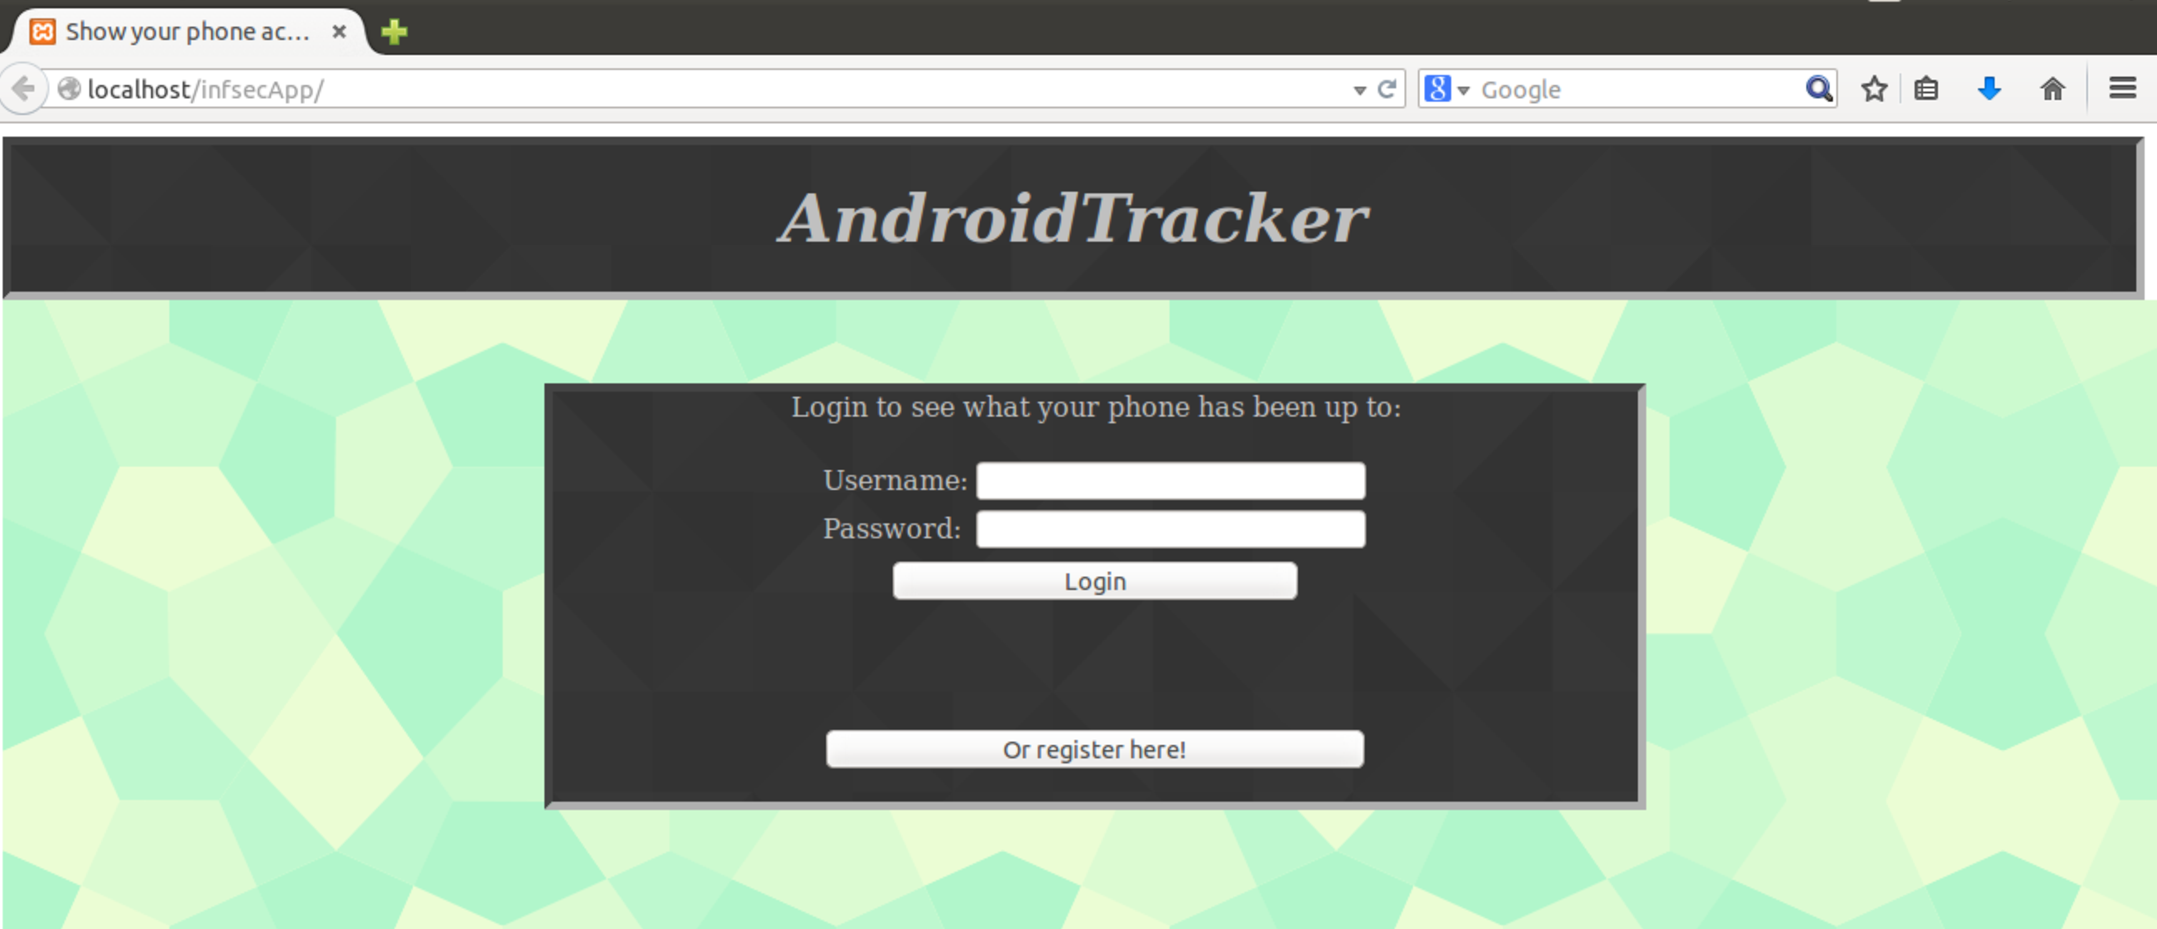
\includegraphics[height=0.4\textheight]{figures/webApp_loginScreen.pdf}
			\end{center}
		\end{itemize}
	\end{frame}

	\begin{frame}
		\frametitle{Web Application - Map Features}
		\begin{itemize}
			\item locations are displayed using Google Map Markers
			\item numbers are written in the markers to indicate the order in which the location data has been received
			\item lines between markers indicate paths
			\item circle around markers indicate accuracy
			\item upon mouse over the time-stamp of the location update as well as the accuracy is shown
			\item map centers around last known location
		\end{itemize}
	\end{frame}

	\begin{frame}
		\frametitle{Web Application - Screenshot}
		\begin{center}
		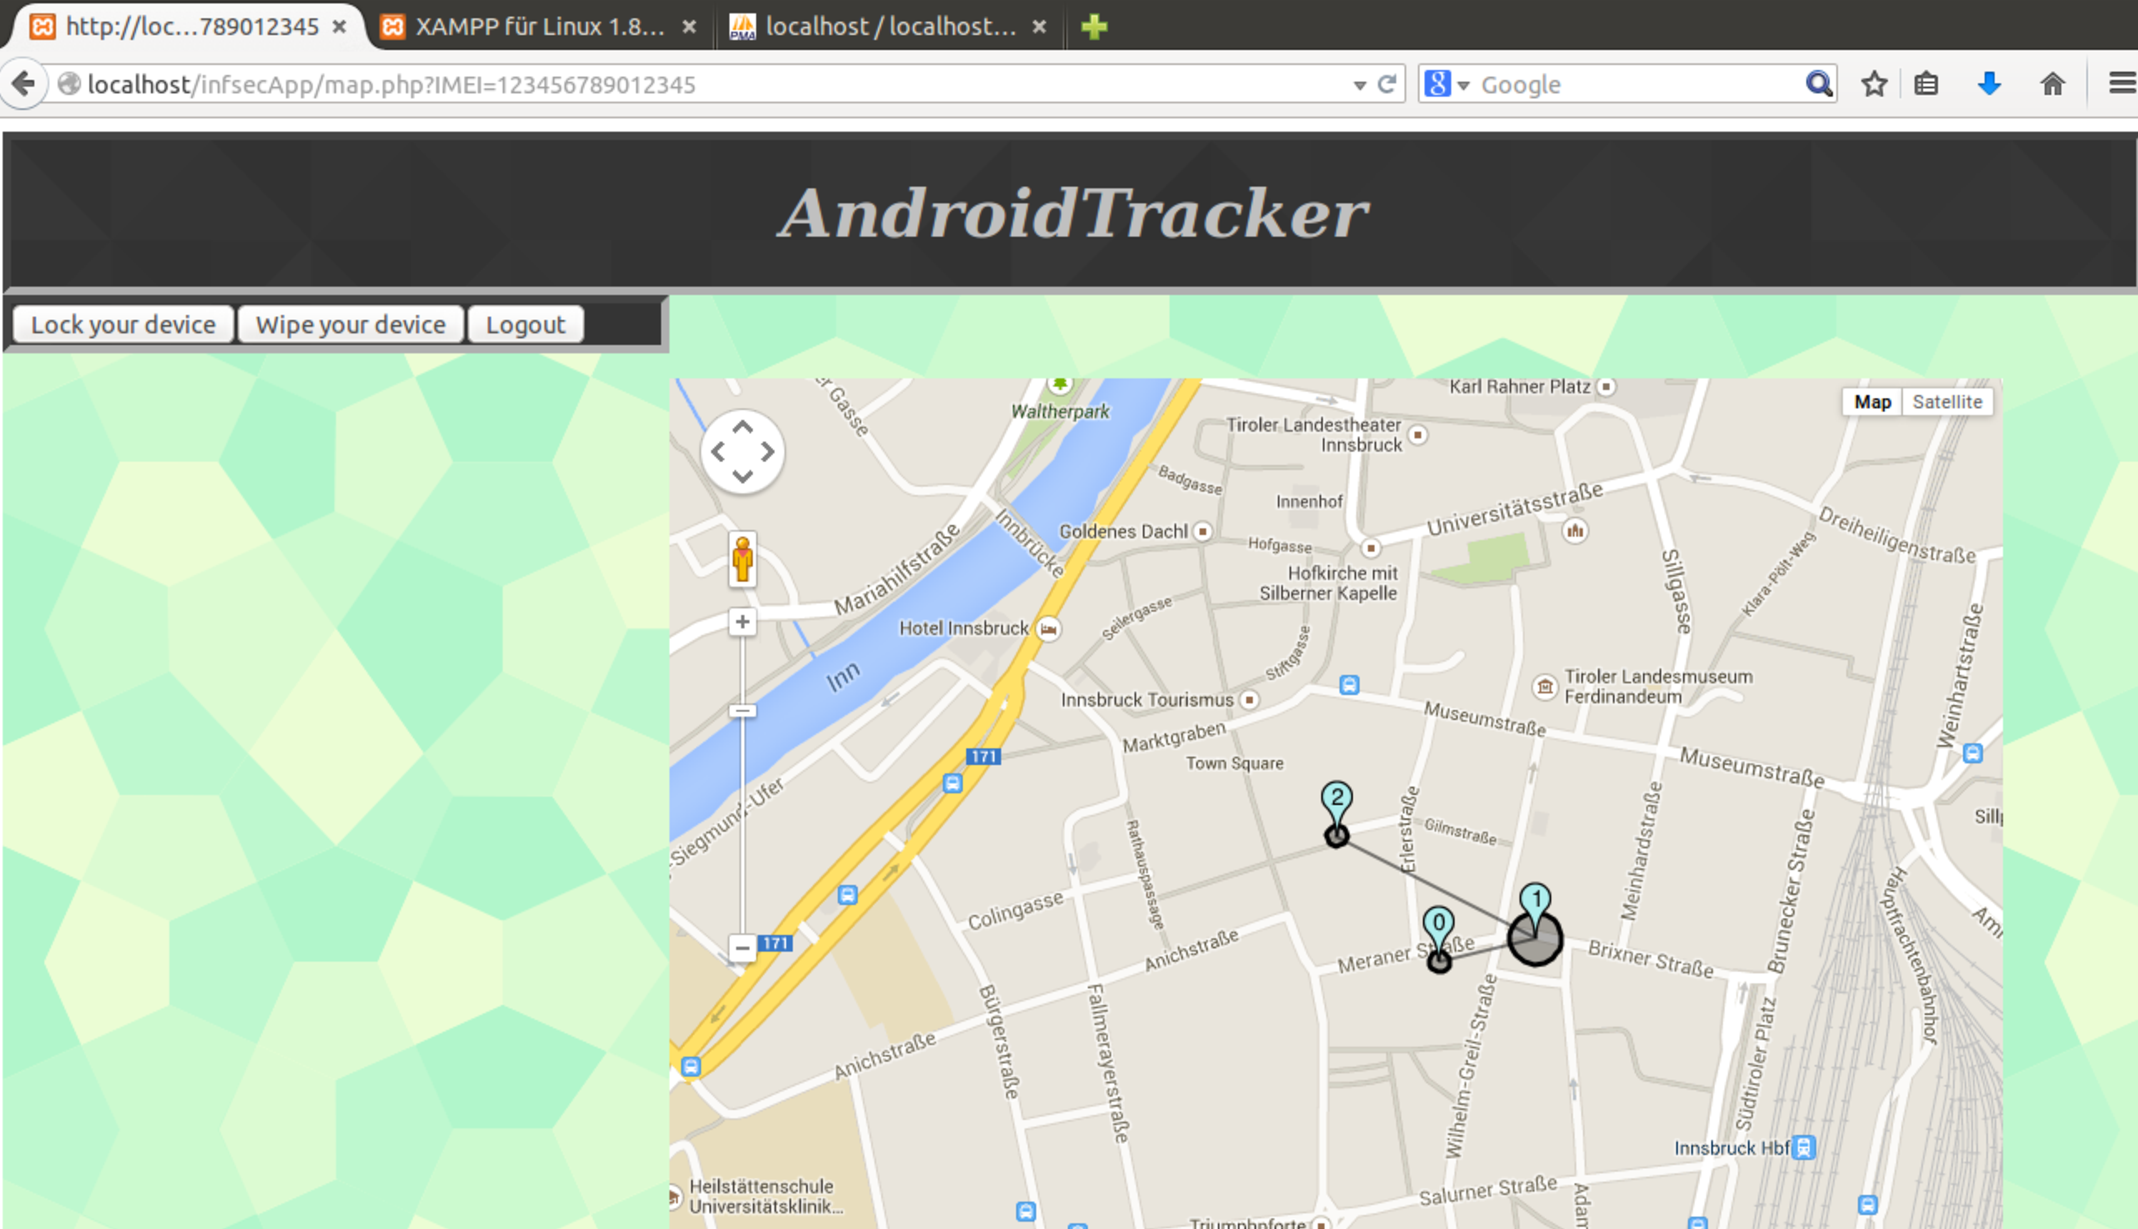
\includegraphics[height=0.75\textheight]{figures/webApp_map.pdf}
		\end{center}
	\end{frame}

	\begin{frame}
		\frametitle{Web Application - Details}
		\begin{itemize}
			\item locking and wiping requests are saved in DB and sent to the user with the next arrival of coordinates
			\item data aggregation:
			\begin{itemize}
			\item received coordinates are compared to last received ones
			\item if difference (in meters) is smaller than a certain threshold (currently 3 meters) the location is not saved in the database, but timestamp of last location is updated
			\end{itemize}
		\end{itemize}
	\end{frame}


	\begin{frame}
		\frametitle{Thank you for your attention!}
		\begin{itemize}
			\item[] \huge{QUESTIONS?}
			\item \normalsize{\url{https://github.com/christophL/AndroidTracker}}
		\end{itemize}
	\end{frame}

	
\end{document}
